
% 1 : x; 2: y; 3: no; 4: tikz object name
\newcommand\smemarbpe[4]{
    \node[rectangle, draw, color=black, thick, anchor=south west, minimum width=1.2cm, minimum height=1cm, inner sep=0pt] (#4) at (#1, #2) {PE#3};
    \node[rectangle, draw, color=black, thick, anchor=south west, minimum width=0.8cm, minimum height=0.5cm, inner sep=0pt] (IC#4) at (#1 + 1.2, #2) {{\small I\$}};
    \node[rectangle, draw, color=black, thick, anchor=south west, minimum width=0.8cm, minimum height=0.5cm, inner sep=0pt] (DC#4) at (#1 + 1.2, #2 + 0.5) {{\small D\$}};
}

% 1 : x; 2: y; 3: tikz object name
\newcommand\smemRRarb[3]{
    \node[circle, draw, color=black, thick, minimum size=0.7cm, inner sep=0pt] (#3) at (#1, #2) {\textit{\scriptsize RR}};
    \draw[ultra thick, ->, >=latex] (#3.west) -- ([yshift=-0.6em]#3.west); 
}

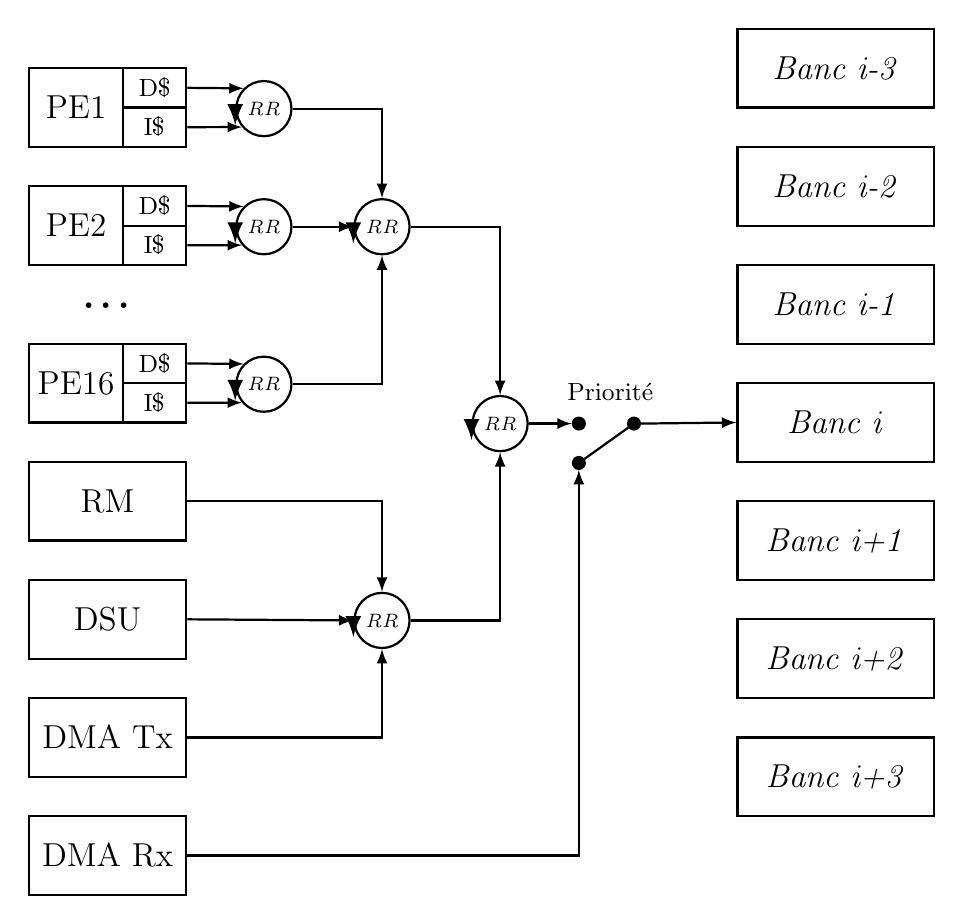
\begin{tikzpicture}[font={\fontsize{12pt}{12}\selectfont}]


    \node[rectangle, draw, color=black, thick, anchor=south west, minimum width=2cm, minimum height=1cm, inner sep=0pt] (DMARx) at (0, 0) {DMA Rx};

    \node[rectangle, draw, color=black, thick, anchor=south west, minimum width=2cm, minimum height=1cm, inner sep=0pt] (DMATx) at (0, 1.5) {DMA Tx};
    \node[rectangle, draw, color=black, thick, anchor=south west, minimum width=2cm, minimum height=1cm, inner sep=0pt] (DSU) at (0, 3) {DSU};
    \node[rectangle, draw, color=black, thick, anchor=south west, minimum width=2cm, minimum height=1cm, inner sep=0pt] (RM) at (0, 4.5) {RM};
    \smemRRarb {4.5}{3.5}{rrRM}
    \draw[thick, ->, >=latex] (RM.east) -| (rrRM.north);
    \draw[thick, ->, >=latex] (DMATx.east) -| (rrRM.south);
    \draw[thick, ->, >=latex] (DSU.east) -- (rrRM.west);

    
    \smemarbpe{0}{6}{16}{pe16}
    \smemRRarb {3}{6.5}{rrpe16}
    \draw[thick, ->, >=latex] (ICpe16.east) -- (rrpe16.220);
    \draw[thick, ->, >=latex] (DCpe16.east) -- (rrpe16.135);
    \node at (1, 7.5) {{\Huge ...}};
    
    \smemarbpe{0}{8}{2}{pe2}
    \smemRRarb {3}{8.5}{rrpe2}
    \draw[thick, ->, >=latex] (ICpe2.east) -- (rrpe2.220);
    \draw[thick, ->, >=latex] (DCpe2.east) -- (rrpe2.135);
    
    \smemarbpe{0}{9.5}{1}{pe1}
    \smemRRarb {3}{10}{rrpe1}
    \draw[thick, ->, >=latex] (ICpe1.east) -- (rrpe1.220);
    \draw[thick, ->, >=latex] (DCpe1.east) -- (rrpe1.135);


    \smemRRarb {4.5}{8.5}{rrPEs}
    \draw[thick, ->, >=latex] (rrpe1.east) -| (rrPEs.north);
    \draw[thick, ->, >=latex] (rrpe2.east) -- (rrPEs.west);
    \draw[thick, ->, >=latex] (rrpe16.east) -| (rrPEs.south);
    
    \smemRRarb {6}{6}{rrFinal}
    \draw[thick, ->, >=latex] (rrPEs.east) -| (rrFinal.north);
    \draw[thick, ->, >=latex] (rrRM.east) -| (rrFinal.south);

    \node[circle, draw, color=black, fill=black, thick, minimum size=0.15cm, inner sep=0pt] (lpint) at (7, 6) {};
    \node[circle, draw, color=black, fill=black, thick, minimum size=0.15cm, inner sep=0pt] (hpint) at (7, 5.5) {};
    \node[circle, draw, color=black, fill=black, thick, minimum size=0.15cm, inner sep=0pt] (outint) at (7.7, 6) {};
    \node at (7.4, 6.4) {{\small Priorité}};
    \draw[thick, ->, >=latex] (rrFinal.east) -- (lpint.west);
    \draw[thick, ->, >=latex] (DMARx.east) -| (hpint.south);
    \draw[thick] (hpint) -- (outint);
    
    \node[rectangle, draw, color=black, thick, anchor=south west, minimum width=2.5cm, minimum height=1cm, inner sep=0pt] (banki) at (9, 5.5) {\textit{Banc i}};
    \node[rectangle, draw, color=black, thick, anchor=south west, minimum width=2.5cm, minimum height=1cm, inner sep=0pt] at (9, 4) {\textit{Banc i+1}};
    \node[rectangle, draw, color=black, thick, anchor=south west, minimum width=2.5cm, minimum height=1cm, inner sep=0pt] at (9, 2.5) {\textit{Banc i+2}};
    \node[rectangle, draw, color=black, thick, anchor=south west, minimum width=2.5cm, minimum height=1cm, inner sep=0pt] at (9, 1) {\textit{Banc i+3}};
    \node[rectangle, draw, color=black, thick, anchor=south west, minimum width=2.5cm, minimum height=1cm, inner sep=0pt] at (9, 7) {\textit{Banc i-1}};
    \node[rectangle, draw, color=black, thick, anchor=south west, minimum width=2.5cm, minimum height=1cm, inner sep=0pt] at (9, 8.5) {\textit{Banc i-2}};
    \node[rectangle, draw, color=black, thick, anchor=south west, minimum width=2.5cm, minimum height=1cm, inner sep=0pt] at (9, 10) {\textit{Banc i-3}};

    \draw[thick, ->, >=latex] (outint.east) -- (banki.west);
    
\end{tikzpicture}
